\documentclass{wsdcr}
\usepackage[backend=bibtex]{biblatex}
\addbibresource{rapport.bib}

\title{Étude du model Lotka-Volterra}
\author{Robin Botrel, Axel Carpentier}
\affil{\textit{Université Paul Sabatier}\\
\textit{Toulouse, France}}
\date{28 Decembre, 2022}

\begin{document}

\maketitle
\tableofcontents
\section{Introduction}

\lettrine{C}{ette} étude des équations de prédation de Lotka-Volterra s'effectue dans le cadre d'une unité d'enseignement ouverte de la licence de mathématique de l'université Paul Sabatier. Nous allons partir d'un exercice vu en cours d'équations différentielles ordinaires (EDO), pour ensuite s'éloigner des frontières de ce cours et voir ce que peut offrir la discipline.



\subsection{Le model classique proie prédateur}

Les équations de Lotka-Volterra qualifient un système d'équations différentielles non linéaires, historiquement développées au début du 20ème siècle pour modéliser les interactions entre espèces et plus particulièrement entre 2 espèces : une proie et un prédateur, elles sont un exemple classique d'EDO. \ref{eq:lotka-volterra} \cite{lotka1920}
\begin{equation}
\left\{
{\begin{array}{ccc}{\dfrac {\mathrm {d} x(t)}{\mathrm {d} t}}&=&x(t)\ {\Big (}\alpha -\beta y(t){\Big )}\\{\dfrac {\mathrm {d} y(t)}{\mathrm {d} t}}&=&y(t)\ {\Big (}\delta x(t)-\gamma {\Big )}\end{array}}
\right.
\label{eq:lotka-volterra}
\end{equation}
\begin{figure}[b!]
\fcolorbox{wsdred}{wsdgrey}{ 
%% first argument is the frame color
%% second argument is the background color
\begin{minipage}{.95\linewidth}
\color{white}

%% the title of the minipage
\begin{center}
    \fontsize{10}{12}\fontfamily{phv}\fontshape{sc}\selectfont
    \textbf{Un peu d'histoire des mathématiques}
\end{center}

%\begin{wrapfigure}{r}{.3\linewidth}
%\includegraphics[width=\linewidth]{}
%\end{wrapfigure}
Dans sa publication de 1920 (la première fois où l'on voit l'équation \ref{eq:lotka-volterra} sous cette forme), Lokta introduit son model comme un simple cas particulier : La source de nourriture de l'espèce 1 (notée $S_1$) est en excès et peut donc être considérée constante sur la période donnée. l'espèce $S_2$ se nourrit alors de $S_1$.
Il introduit son raisonnement, $X_1$ est la masse de l'espèce $S_1$  :
\begin{equation}
\begin{aligned}
&\begin{bmatrix}
\text{Variation de }X_1 \\ \text{par unité de temps}
\end{bmatrix}
=
\begin{bmatrix}
X_1\text{ engendré}\\ \text{par unité de temps}
\end{bmatrix} \\
&- 
\begin{bmatrix}
X_1\text{ détruit par }X_2\\ \text{par unité de temps}
\end{bmatrix}
-
\begin{bmatrix}
\text{autre perte de }X_1\\ \text{par unité de temps}
\end{bmatrix} \\
&\begin{bmatrix}
\text{Variation de }X_2 \\ \text{par unité de temps}
\end{bmatrix}
=
\begin{bmatrix}
X_2\text{ engendré par l'ingestion de }X_1\\ \text{par unité de temps}
\end{bmatrix} \\
&-
\begin{bmatrix}
\text{autre perte de }X_2\\ \text{par unité de temps}
\end{bmatrix} 
\end{aligned}
\end{equation}
Pour translater ce raisonnement en un système d'EDO, il va faire de nouvelles assomptions.
$\ll$ Pour de petits changements, le taux de formation de nouvelle matière d'une espèce donnée d'organisme dans des conditions déterminées est proportionnel à la masse existante de cette espèce. En d'autres termes, la croissance de la matière vivante est un processus typiquement 'autocatakinetic'. […]. La proportionnalité ne s'applique pas aux grandes variations de X1, X2, ce qui est dûment pris en compte dans la mesure où $A_1'$, est une fonction de X1, X2. […]. De même, la masse de S1 détruite par S2 qui s'en nourrit sera, pour de petites variations, proportionnelle à X2 et aussi à X1. Ce terme a donc été défini sous la forme BiXiX2. Ici encore, les écarts de proportionnalité sont pris en charge par les variations de B1 avec X1 et X2, variables dont B1 est une fonction. $\gg$
\begin{equation}
\begin{aligned}
{\dfrac {\mathrm {d} X_1(t)}{\mathrm {d} t}}&=A_1'X_1-B_1X_1X_2-A_1"X_1\\
{\dfrac {\mathrm {d} X_2(t)}{\mathrm {d} t}}&=A_2X_1X_2-B_2X_2
\end{aligned}
\end{equation}
Il se base sur l'idée de proportionnalité et traite AB comme des fonctions durant toute la publication. C'est Volterra qui en 1926 dans des lettres à Umberto D'Ancona, décrit la même équation mais tel que AB soit fixes, il semble ne pas connaître les résultats de Lotka.
\end{minipage}
}
\end{figure}
\subsection{Généralisation}
\begin{equation}
\left\{
{\begin{array}{ccc}{\dfrac {\mathrm {d} x(t)}{\mathrm {d} t}}&=&x(t)\ {\Big (}a -b y(t)-c x(t){\Big )}\\{\dfrac {\mathrm {d} y(t)}{\mathrm {d} t}}&=&y(t)\ {\Big (}d x(t)-e -f y(t) {\Big )}\end{array}}
\right.
\end{equation}
\begin{equation}
\dfrac {\mathrm {d}}{\mathrm {d} t}X(t)=X(t) {\Big (}R+AX(t){\Big )}
\end{equation}
\section{Le cas 2D}
\subsection{Champ vectoriel}
\subsection{Une étude des bifurcations}
\begin{equation}
R={\begin{bmatrix}1\\1\end{bmatrix}}\quad A =-{\begin{bmatrix}1&1\\1&1\end{bmatrix}}
\end{equation}
\begin{equation}
R={\begin{bmatrix}1\\1\end{bmatrix}}\quad A =-{\begin{bmatrix}1&s\\s&1\end{bmatrix}}
\end{equation}
\section{Chaos en 4D}
\subsection{introduction aux attracteurs}
\begin{equation}
R={\begin{bmatrix}1\\0.72\\1.53\\1.27\end{bmatrix}}\quad A =-{\begin{bmatrix}1&1.09&1.52&0\\0&0.72&0.3168&0.9792\\3.5649&0&1.53&0.7191\\1.5367&0.6477&0.4445&1.27\end{bmatrix}}
\end{equation}
\subsection{bifurcations}
\begin{equation}
R={\begin{bmatrix}1\\0.72\\1.53\\1.27\end{bmatrix}}\quad A =-{\begin{bmatrix}1&1.09s&1.52s&0\\0&0.72&0.3168s&0.9792s\\3.5649s&0&1.53&0.7191s\\1.5367s&0.6477s&0.4445s&1.27\end{bmatrix}}
\end{equation}
\begin{figure}[t!]
    \centering
    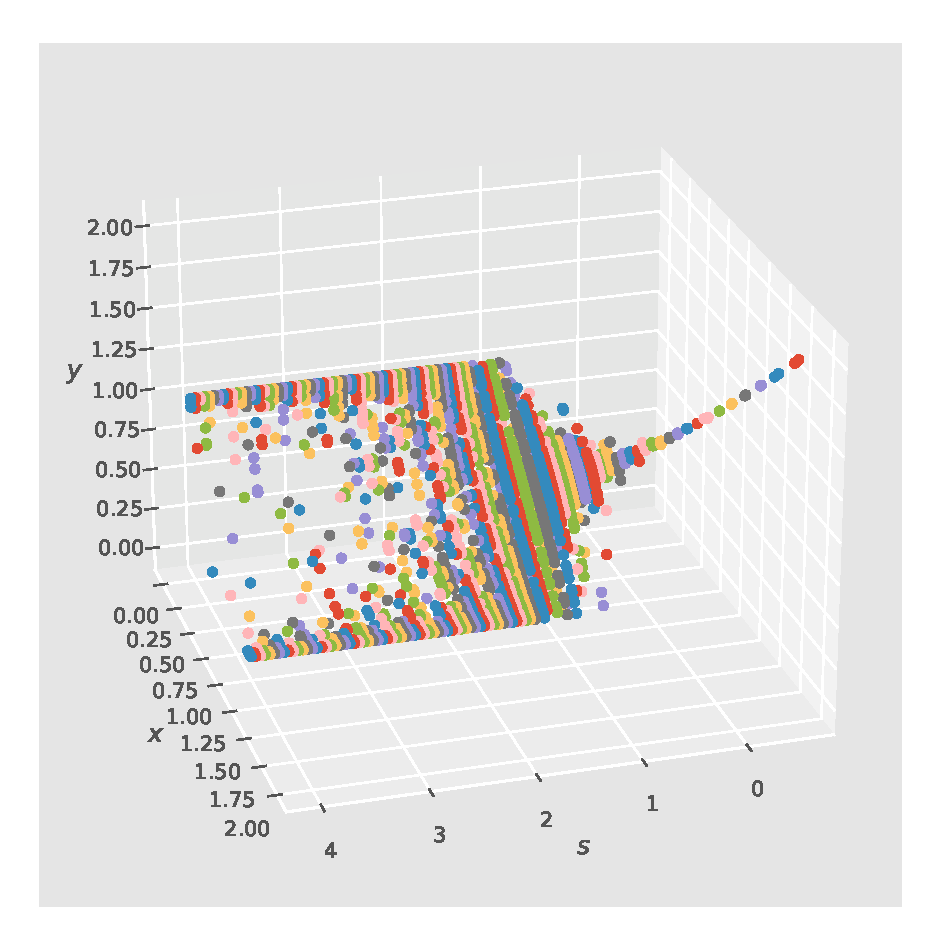
\includegraphics[width=\linewidth]{fig/lv2_bif3D.eps}
    \caption{test}
    \label{fig:example}
\end{figure}
\subsection{Cycle limite}
\begin{equation}
R={\begin{bmatrix}1\\0.72\\1.53\\1.27\end{bmatrix}}\quad A =-{\begin{bmatrix}1&1.0355&1.444&0\\0&0.72&0.30096&0.93024\\3.386655&0&1.53&0.683145\\1.459865&0.615315&0.422275&1.27\end{bmatrix}}
\end{equation}
\begin{figure}[t!]
    \centering
    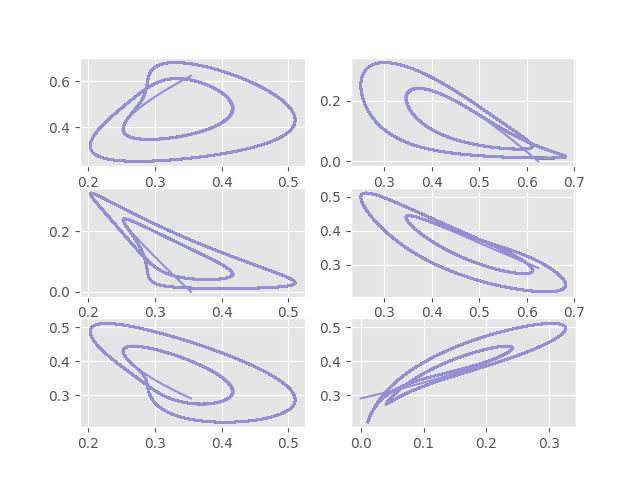
\includegraphics[width=\linewidth]{fig/lv4_cl.png}
    \caption{test}
    \label{fig:example}
\end{figure}
\subsection{Exposant de Liapounov}
\section{Conclusion}

\section{Annexes}
\section{bibliographie}
\nocite{*}
\printbibliography
%An example of a figure is shown in Figure \ref{fig:example}. The recommended width of the figure is $0.9\times$\textbackslash linewidth, and the recommended width:height aspect ratio is $1.41:1$ (i.e. A4 paper)
%
%Additionally, one can create a minipage for extra information like biography as shown in the following:
%
%\footnotetext[1]{acquired from the official website of IPS at\\https://www.waseda.jp/fsci/gips/en/about/overview-2/}
%
%%\begin{figure}[t!]
%%    \centering
%%    \includegraphics[width=.9\linewidth]{}
%%    \caption{The logo of IPS, Waseda University.}
%%    \label{fig:example}
%%\end{figure}
%
%\begin{figure}[b!]
%\fcolorbox{wsdred}{wsdgrey}{ 
%%% first argument is the frame color
%%% second argument is the background color
%\begin{minipage}{.95\linewidth}
%\color{white}
%
%%% the title of the minipage
%\begin{center}
%    \fontsize{10}{12}\fontfamily{phv}\fontshape{sc}\selectfont
%    \textbf{About the School}
%\end{center}
%
%%\begin{wrapfigure}{r}{.3\linewidth}
%%\includegraphics[width=\linewidth]{}
%%\end{wrapfigure}
%\textbf{Waseda University Graduate School of Information, Production and Systems (IPS)} is a graduate school that has no corresponding undergraduate department established within the Kitakyushu Science and Research Park area in 2003 as the base for Waseda University to expand its presence in Asia. With three fields of study, including Information Architecture, Production System, and Integrated Systems, IPS undertakes academic research in the technological fields that society currently requires, and strives to attain a sustainable society through the use of technology. \footnotemark[1].
%\end{minipage}
%}
%\end{figure}
%
%\subsection{Tables}
%Creating tables is the same as any other latex documents, as shown in Table \ref{tab:example}.
%
%\begin{table}[t!]
%    \centering
%    \begin{tabular}{ccc}
%    \hline
%        header1 &  header2 & header 3\\
%        \hline
%        data1 & data2 & data3\\
%        data4 & data5 & data6
%    \end{tabular}
%    \caption{An example of a floating table.}
%    \label{tab:example}
%\end{table}
%
%\section{Equations}
%Just normally input your equations as either inline one: $E=h\frac{\lambda}{c}$ or with equation environment (equation* to remove numbering):
%
%\begin{equation}
%\left\{
%\begin{aligned}
%    &\oiint_{\partial\Omega}{\mathbf{E}\cdot d\mathbf{S}}=\frac 1{\varepsilon_0}\iiint_\Omega{\rho dV}\\
%    &\oiint_{\partial\Omega}{\mathbf{B}\cdot d\mathbf{S}}=0\\
%    &\oint_{\partial\Sigma}{\mathbf{E}\cdot d\boldsymbol{l}}=-\frac d{dt} \iint_\Sigma{{\mathbf{B}\cdot d\mathbf{S}}}\\
%    &\oint_{\partial\Sigma}{\mathbf{B}\cdot d\boldsymbol{l}}=\mu_0 \left(\iint_\Sigma{{\mathbf{J}\cdot d\mathbf{S}}}+\varepsilon_0\frac d{dt} \iint_\Sigma{{\mathbf{E}\cdot d\mathbf{S}}}\right)\cite{Maxwell1865}
%\end{aligned}
%\right.
%\end{equation}
%
%\appendices


\end{document}
